As our differentiable basis set framework lets us differentiate through the whole basis set fitting procedure, we can choose to replace the constant basis functions that are commonly used in DFT calculation with adaptive ones which can adapt to the local chemical environment. \\
Recently there have been new approaches in the field of adaptive basis functions. Fu et. al. \cite{fu_recipe_2024} used an equivariant Graph neural network to prodict the coefficients and exponents for the linear basis for ground state densities of molecules. Schütt et. al.\cite{schutt_machine_2018} used a gaussian process to predict the contraction coefficients of an minimal basis set and recorded significant improvements in the application for DFT simulation. Similarly another approach by Müller et. al.\cite{muller_atom--molecule_2023} used a linear model to predict contraction coefficients for minimal basis sets to improve geometry optimizations and DFT computations carried out on these basis sets.\\
Adaptive exponents inside the Gaussian basis functions have been avoided so far for Kohn Sham DFT calculations as they require one to differentiate through the integrals.
But now owr framework allows us to learn the coefficients and exponents used in basis sets of DFT calculations jointly.
We mainly restrict our analysis to minimal basis sets, specifically the STO-3G and the STO-6G minimal basis sets, as they are expected to profit the most from these improvements.
We then use a small graph neural network, as described in \ref{model} to predict the exponents and coefficients of these Basis sets.
\section{Multi Step Pretraining}
As the differentiable basis functions are currently very slow and use a lot of video random access memory (VRAM) on the GPU, compared to what is common in machine learning, we cannot reach a very high number of iterations in learning.
To compensate for this we're using multiple pretraining procedures to improve the speed at which the neural network is learning.
At first we let the network predict atomwise features, which don't require an evaluation of the differentiable integrals and can therefor be evaluated very quickly.
\subsection{Pretraining on atomwise properties}
We first evaluate the Neural network on atomwise properties to let it learn a kind of "physical intuition" before letting it work on the hard task of reliable predicting coefficients and exponents for each atom.
For the features, we want to predict, we borrow from the labels that have been produced for the orbital free model.
We predict the features by adding an extra linear output head at the last layer of the neural network.\\
The following feature were predicted:\\
\begin{enumerate}
    \item Atomic number of each atom, $Z_i$.
    \item Coulomb potential from each neighboring atom, $-\sum\limits_{a \in \mathcal{N}(i)} \frac{Z_a}{|e_{i-a}|}$.
    \item Sum of Coulomb forces acting on the current atom, $\sum\limits_{a \in \mathcal{N}(i)} \frac{Z_a Z_i}{|e_{i-a}|^2}$.
    \item Effective number of electrons, $\sum\limits_{\mu} \text{mask}(i)_\mu p_\mu w_\mu$.
    \item Effective charge: Atomic number minus the effective number of electrons.
    \item Gradients of the kinetic, external, Hartree, exchange-correlation and total energy integrated over the basis functions centered around each atom individually.
\end{enumerate}
Where $\text{mask(i)}_\mu =
\begin{cases}
1, & \text{if } \omega_\mu(\mathbf{r}) \text{ is centered on } \mathbf{R_i} \\
0, & \text{else}
\end{cases}$.
In praxis this type of pretraining is very fast, as it involves no integrals and can be run with a high batch size, compared to the following methods.
\subsection{Orbitals Deltalearing to bigger basis set}
For the main training step we train the basis set by fitting the orbitals produced by the largely bigger basis set 6-31G(2df,p) with the smaller adaptive basis set.
We define our loss as the sum of the L2 norms between the orbitals produced by the bigger basis set and the orbitals which of the smaller basis set which we fit to the bigger basis set using density fitting.
As the orbitals should be orthonormal to each other we also enforce this property during density fitting.
The loss function is defined as
\begin{align}
    \text{Loss}(\Phi') = \underset{\{\phi_i\}_{i=1,...,N_e} \text{pairwise orthonormal}}{\text{min}}\sum\limits_{i=1}^{N_e} \int (\phi_i(\mathbf{r})-\phi'_i(\mathbf{r}))^2 d\mathbf{r}.
\end{align}
Where $\Phi' = \{\phi'_i\}_{i=1,...,N_e}$ are the occupied orbitals produced by the bigger basis set and $\Phi = \{\phi_i\}_{i=1,...,N_e}$ are the orbitals defined on the basis functions of our smaller basis  which are fitted to the bigger basis set.
The solution of this equation in components leads us to equation \eqref{adaptive_loss_final}.
The derivation of this equation can be found in appendix \ref{derivation_adaptive_loss}, it is identical to the common procedure of data whitening applied to the original orbitals.
\begin{align}\label{adaptive_loss_final}
    \text{Loss} &= \sum_i C_{i,\mu} \langle\eta_\mu|\eta_\nu\rangle C_{i,\nu} - 2 C_{i,\mu} \langle\eta_\mu|\tilde\eta_\nu\rangle \tilde C_{i,\nu} + \tilde C_{i,\mu} \langle\tilde \eta_\mu|\tilde \eta_\nu\rangle \tilde C_{i,\nu}\\
     C_{i,\mu}&= \sum_{j} A^{-\frac{1}{2}}_{i,j} \langle\eta_\mu|\eta_\nu\rangle^{-1}_{\mu,\nu} \langle\eta_\nu|\tilde\eta_\gamma\rangle \tilde C_{j,\gamma}\\
    A_{i,j}&=\tilde C_{i,\sigma}\langle\tilde \eta_\sigma|\eta_\mu\rangle \langle\eta_\mu|\eta_\nu\rangle^{-1}_{\mu,\nu} \langle\eta_\nu|\tilde\eta_\gamma\rangle \tilde C_{i,\gamma}
\end{align}
As we now have a formulation for the loss in terms of simple basis integrals, we can insert the dependency of the integrals on the contraction coefficients $\mathbf{A}$ and exponents $\mathbf{\alpha}$ and their respective dependency on the parameters of the neural network, which we will denote as $\Omega$, as well as the molecule geometry $\mathcal{M}$.\\
Affected are the symmetric overlap matrices $\langle\eta(\alpha[\mathcal{M},\Omega],A[\mathcal{M},\Omega])_\mu|\eta(\alpha[\mathcal{M},\Omega],A[\mathcal{M},\Omega])_\nu\rangle$ and the asymmetric overlap matrices $\langle\eta(\alpha[\mathcal{M},\Omega],A[\mathcal{M},\Omega])_\mu|\tilde \eta_\nu\rangle$.
The overlap matrices of the target basis $\langle\tilde \eta_\mu|\tilde \eta_\nu\rangle$ have no further dependencies and can therefore be omitted from the loss.\\
From here on out, we can train the model, as we did in the previous section, using stochastic gradient descent on the dataset QM9 to minimize the loss function.

\subsection{Gradient Descent on Total Energy}
Training the model to provide basis functions which can produce densities closer to those of the larger basis set is a good start, as, in theory, it lets Kohn-Sham generate better orbitals and therefore also better energies.
But as our adaptive basis set is much smaller than the one we are using as reference, there is a limit to how well the orbitals can be fitted.
Even worse, trying to fit the densities too closely could lead to unphysical basis functions which produce better fits but worse energies.\\ If we want to optimize our predicted basis sets to produce better energies, we should optimize the total energy directly.
As we want to predict the ground state energy of a molecule, which means the state with the lowest energy, we want to find the basis set which produces the lowest energy.
We can therefore use the total energy as a loss function.
The total energy in Kohn-Sham is defined as
\begin{align}
    E_{\text{tot}}[\Phi] = T_S[\Phi] + V_{\text{ext}}[\Phi] + V_{\text{H}}[\Phi] + V_{\text{xc}}[\Phi] + E_{\text{NN}}.
\end{align}
Our differentiable integrals let us compute each of these functions in a differentiable way and insert our dependencies on the contraction coefficients, the exponents, and lastly the parameters of the neural network.
However, we also need to keep in mind that the orbitals calculated by Kohn-Sham $\Phi = {\phi_i}_{i=1,...,N_e}$ are also dependent on these parameters. \\
Let us now insert these dependencies and perform the derivative with respect to the model parameters:

\begin{align}
    E_{\text{tot}}[\Phi(\alpha[\mathcal{M},\Omega],&A[\mathcal{M},\Omega]),\alpha[\mathcal{M},\Omega],A[\mathcal{M},\Omega]] \\
    &= T_S[\Phi(\alpha[\mathcal{M},\Omega],A[\mathcal{M},\Omega]),\alpha[\mathcal{M},\Omega],A[\mathcal{M},\Omega]] \nonumber\\
    &+ V_{\text{ext}}[\Phi(\alpha[\mathcal{M},\Omega],A[\mathcal{M},\Omega]),\alpha[\mathcal{M},\Omega],A[\mathcal{M},\Omega]] \nonumber\\
    &+ V_{\text{H}}[\Phi(\alpha[\mathcal{M},\Omega],A[\mathcal{M},\Omega]),\alpha[\mathcal{M},\Omega],A[\mathcal{M},\Omega]] \nonumber\\
    &+ V_{\text{xc}}[\Phi(\alpha[\mathcal{M},\Omega],A[\mathcal{M},\Omega]),\alpha[\mathcal{M},\Omega],A[\mathcal{M},\Omega]] + E_{\text{NN}}\nonumber\\
        \frac{\partial E_{\text{tot}}[...]}{\partial \Omega}
    &= \frac{\partial E_{\text{tot}}[...]}{\partial \phi_i[...]}\frac{\partial \phi_i[...]}{\partial \Omega} + \frac{\partial E_{\text{tot}}[...]}{\partial \alpha[...]}\frac{\partial \alpha[...]}{\partial \Omega} + \frac{\partial E_{\text{tot}}[...]}{\partial A[...]}\frac{\partial A[...]}{\partial \Omega}
\end{align}
If we now choose the orbitals to be ground state orbitals of the current basis set, then by definition the derivative of the total energy with respect to the orbitals is zero $\frac{\partial E_{\text{tot}}[...]}{\partial \phi_i[...]}=0$.
This means that we can remove the dependency of the orbitals on the model parameters and can still calculate the gradient of the total energy with respect to the model parameters. \\
We therefore propose the following training scheme: \\
First, we use the current model to predict the basis for our current molecule.
Then we fix this basis and use PySCF's\cite{sun2020recent} implementation of Kohn-Sham to compute the ground state orbitals in a non-differentiable way.
Now we take these orbitals and, using our differentiable integrals framework, calculate the total energy of the molecule with enabled autograd.\\
We can then use the calculated total energy as our loss function for which we can calculate the gradient with respect to the model parameters.
Lastly we can use gradient descent to update the parameters of the model.
This way we can apply stochastic gradient descent to minimize the total energies of the molecules in the QM9 dataset.\\


The major drawback of this approach is that it needs a complete Kohn-Sham calculation in each step, and the calculation of the total energy using the differentiable integrals is also very slow and requires a lot of RAM. To lower the load, we used density fitting using the Hartree fitting method with an even-tempered 3.0 basis set built on our minimal basis set to emulate the calculation of the Hartree energy $E_H$. \\
Even with these improvements, we could only run a single calculation on a GPU at a time while also strongly utilizing the CPU. We therefore could only run a few iterations of this training scheme.


\subsection{Combination of the Individual Steps}
When trying to train a randomly initialized model or one pretrained on atomic properties, we found that the initial variations in the predicted exponents and coefficients were often too large and led to catastrophic failure in the fitting of the orbitals or Kohn-Sham calculations.\\
Our solution to this problem is the following: Before starting to train the model to predict the exponents and coefficients for basis functions, we collect the statistics for each output head for the first 100 molecules and then add a layer to the output head which subtracts the calculated mean and divides by its found standard deviation. \\
These weights are then fixed for the rest of the training.
This way we ensure that the predicted exponents and coefficients are in a reasonable range and the model can start to learn the more subtle dependencies of the basis functions first.
This led to much stabler training and reduced the number of catastrophic failures.
Still, it was necessary to use a very small learning rate to minimize the risk of exploding gradients.\\
We found that pretraining the model on atomic properties is not necessary to achieve good results.
But using pretraining speeds up the following delta-learning to a bigger basis set or gradient descent on the total energy procedures significantly.
We also tried additional side losses, similar to those in the previous section, but found their effect negligible.
We will now evaluate and compare the best few models we trained using the mentioned procedures:
\begin{enumerate}
    \item adaptive\_STO-6G\_0: Based on STO-6G Used pretraining and delta learning to 6-31G(2df,p).
    \item adaptive\_STO-6G\_1: Based on STO-6G Used pretraining and delta learning to 6-31G(2df,p).
    \item adaptive\_STO-3G\_0: Based on STO-3G Used pretraining and delta learning to 6-31G(2df,p).
    \item adaptive\_STO-3G\_1: Based on STO-3G Used pretraining, delta learning to 6-31G(2df,p) and gradient decent on the total energy.
    \item adaptive\_STO-3G\_2: Based on STO-3G Used pretraining and delta learning to 6-31G(2df,p).
    \item adaptive\_STO-3G\_3: Based on STO-3G Used pretraining and delta learning to 6-31G(2df,p).
\end{enumerate}
\Section{Evaluation}
To evaluate our adaptive basis sets, we selected 210 molecules evenly distributed over QM9 and ran full spin-restricted Kohn-Sham calculations to obtain ground state densities and energies.
As a point of reference, we also ran calculations for the minimal basis sets STO-3G and STO-6G, as well as non-minimal basis sets 3-21G, 4-31G, 6-31G, and 6-31G(2df,p).
We then compared the results of the adaptive basis sets to the reference calculations.\\


In Figure \ref{fig:classical_exps_coeffs}, we depicted the exponents and coefficients of these basis sets and their contraction into basis functions.
We can note that the larger basis sets mainly have a higher number of basis functions and basis functions with higher angular momentum, while they do not significantly increase the number of primitive basis functions. For example, 3-21G has the same number of primitive basis functions as STO-36 but contracts them into a higher number of basis functions.
This leads to the basis being more flexible but also slows down Kohn-Sham calculations as it increases the size of the Fock matrix.\\


In theory, our learned adaptive basis sets could achieve accuracy close to 3-21G but with the speed of STO-3G. This makes 3-21G very useful for comparison.
We are going to compare the adaptive basis sets to the reference calculations using the following metrics:\\

\begin{enumerate}
    \item Absolute Error (AE) of the Energies (Hartree, External, xc) compared to  6-31G(2df,p).
    \item The L2 Norm of the difference in densities $\text{L2}[\rho-\rho'] = \sqrt{\int (\rho(\mathbf{r})-\rho'(\mathbf{r}))^2} d\mathbf{r}$
    \item The L1 Norm of the difference in densities $\text{L1}[\rho-\rho'] = \int |\rho(\mathbf{r})-\rho'(\mathbf{r})| d\mathbf{r}$.
\end{enumerate}
Where $\rho(\mathbf{r} ) = (\sum_i^{N_e} \phi_i(\mathbf{r}))^2$ is the density produced by the kohn sham orbitals, and $\rho'(\mathbf{r}) = (\sum_i^{N_e} \phi'_i(\mathbf{r}))^2$ is the density produced by the reference orbitals of 6-31G(2df,p).
As in quantum chemesty the absolute energies are not as important as the relative energies we also compare the relative errors of the energies.
We compute the relative error of the energies as
\begin{align}\label{relative_energy_errors}
    \text{AE}_{\text{relative energy } \cdot} [\Phi]  &= \frac{1}{N_{mol}}\sum_{j=1}^{N_{mol}}\text{Abs}\left((E_\cdot[\Phi]-E_\cdot[\Phi_j])-(E_\cdot[\Phi']-E_\cdot[\Phi'_j])\right).
\end{align}
Where we calculate the relative difference in energy between a sample molecule $E_\cdot[\Phi]$ and the energies of all other molecules in the test set $\{E_\cdot[\Phi_j]\}_{j=1,...,N_e}$ and compare this difference to the differences which are produced by the reverence basis $\{(E_\cdot[\Phi']-E_\cdot[\Phi'_j])\}_{j=1,...,N_e}$. \\

We than take the mean of the absolute value of these differences.
These relative energies are more valuable than absolute energies, as a constant shift in energy, which would chemically make no difference to the system, also doesn't affect the relative energies.
\section{Results}
In figure\ref{fig:AE_energies_adaptive_basis_sets} we can see the absolute energy differences of the fitted basis sets to 6-31G(2df,p).
Our first observation is that the bigger basis sets also have a lower MAE for the total energy than the smaller ones.
For the external energy and the exchange correlation energy this is no longer true. \\
We can find a slight trend to lower MAE for smaller basis sets, but as it is the objective of kohn sham to minimize the total energy , the contribution of the other densities may vary more strongly.
For the fitted basis sets we also find that adaptive\_STO-3G\_0-3 slightly improve on STO-3G in terms of the total energy, but produce much worse external and exchange correlation energies.
They also dont manage to catch up to the bigger basis sets. adaptive\_STO-6G\_0 and adaptive\_STO-6G\_1 on the other side, while having the same number of basis functions as STO-3G, can improve significantly on STO-6G with the total energy and even surpas 4-31G. They also manage to improve on STO-6G on the external and exchange correlation energy.\\
\begin{figure}
    \centering
    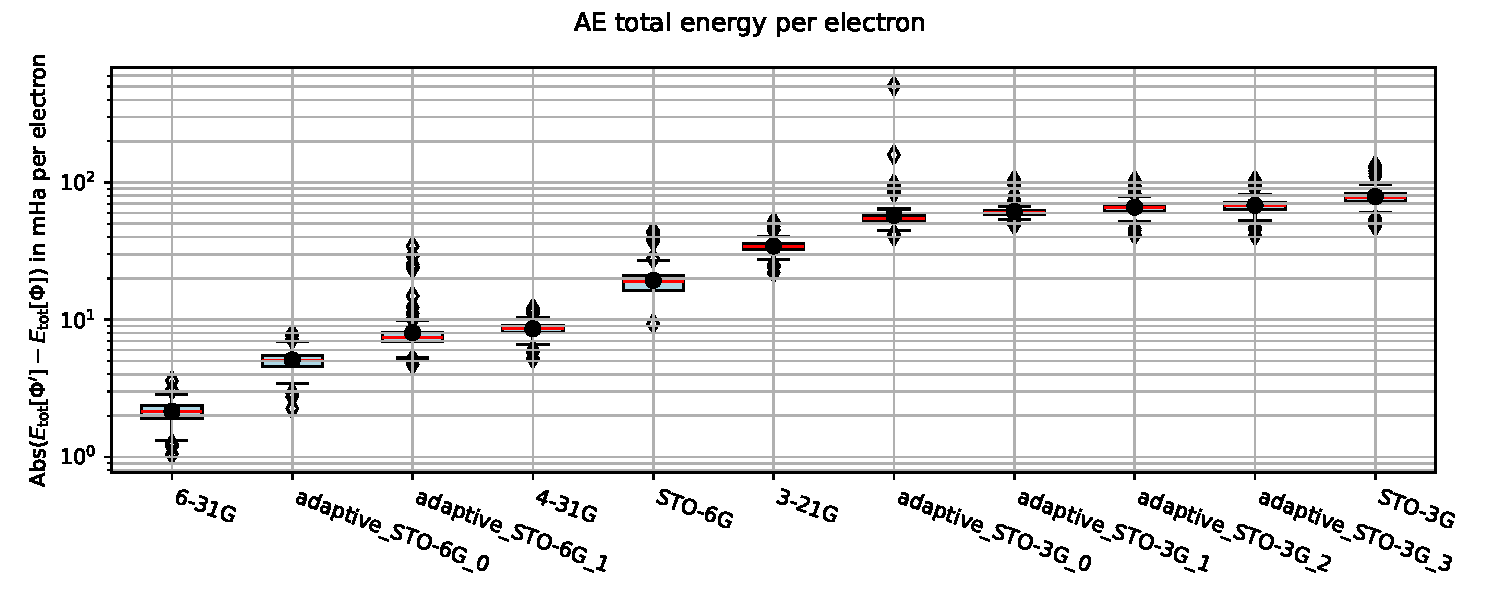
\includegraphics[width=0.9\textwidth]{chapters/results/results_images/adaptive_basis_functions/total_energy_adaptive_basis_sets}
    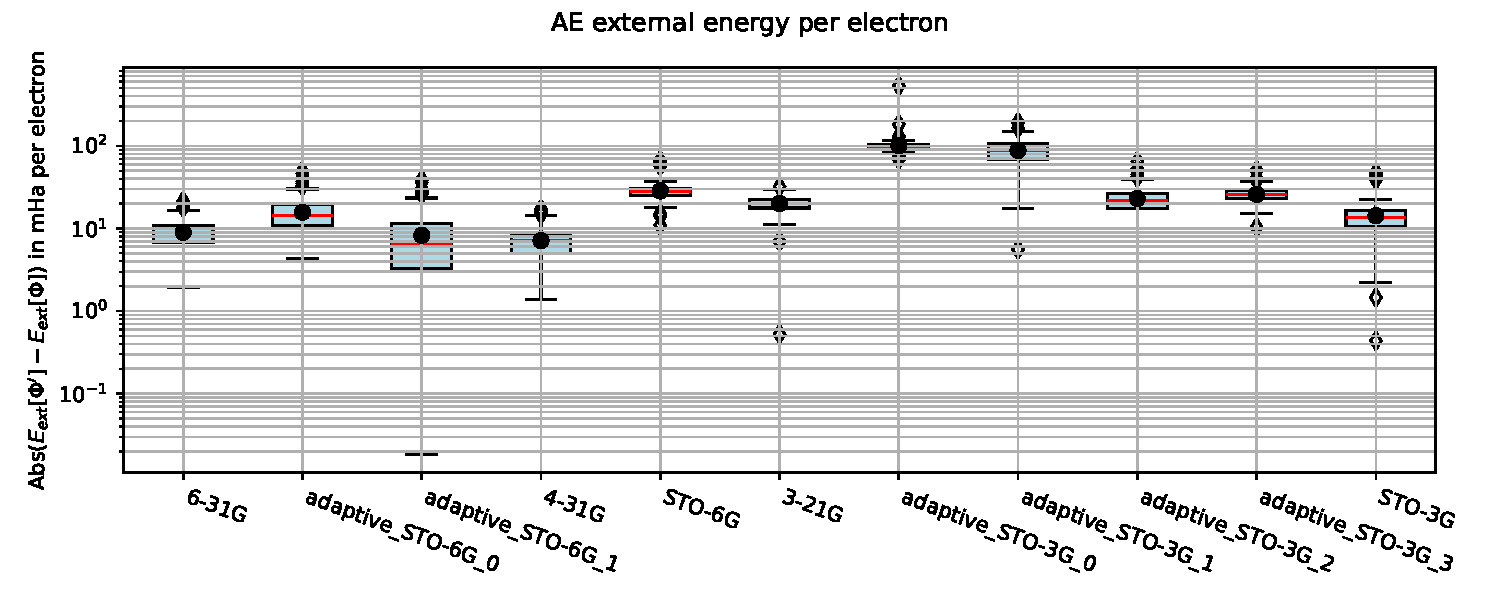
\includegraphics[width=0.9\textwidth]{chapters/results/results_images/adaptive_basis_functions/coulomb_energy_adaptive_basis_sets}
    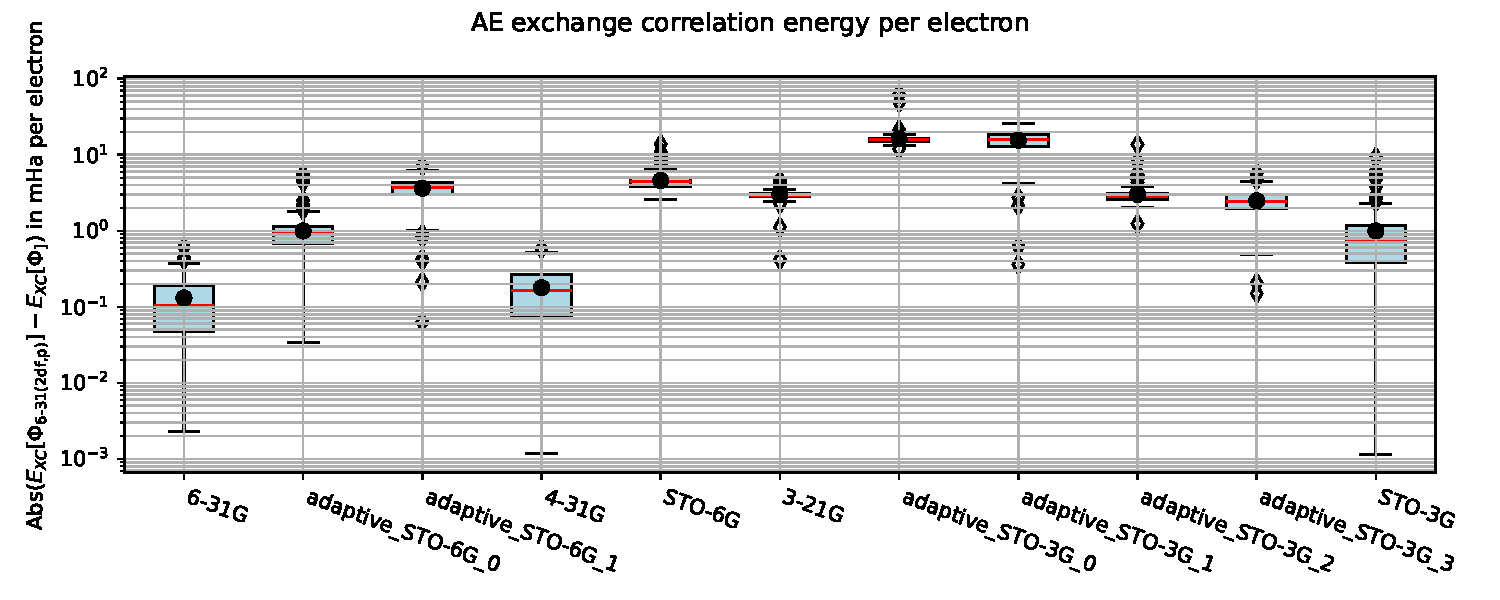
\includegraphics[width=0.9\textwidth]{chapters/results/results_images/adaptive_basis_functions/exchange_correlation_energy_adaptive_basis_sets}
    \caption{Boxplots(\ref{boxplots}) of the AE for the different energies produced by kohn sham on the different classical and adaptive basis functions on 210 Molecules evenly distributed over QM9, compared to calculations on the basis set "6-31G(2df,p)".} \label{fig:AE_energies_adaptive_basis_sets}
\end{figure}
Next of we are going to compare the relative energy values depicted in figure \ref{fig:AE_relative_energies_adaptive_basis_sets}.
For the total energy the ranking of the basi sets stays mostly the same, exept for adaptive\_STO-6G\_1 and 4-31G, which swap places.
It seems that while adaptive\_STO-6G\_1 produces the slightly better absolute total energy, 4-31G produces the better relative total energy. For the external and exchange correlation energy we find the same behavior as before for the absolute energies.\\
\begin{figure}
    \centering
    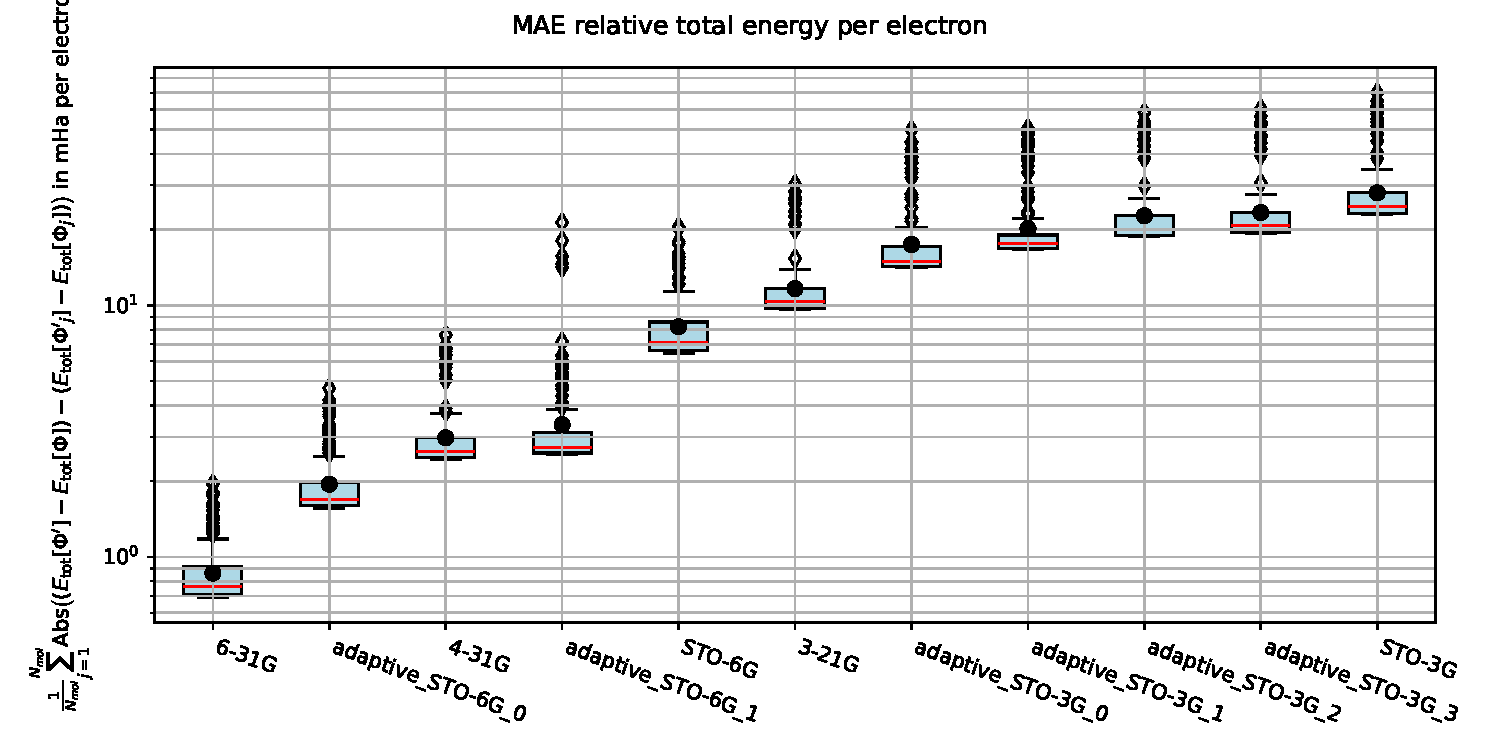
\includegraphics[width=0.9\textwidth]{chapters/results/results_images/adaptive_basis_functions/relative_total_energy_adaptive_basis_sets}
    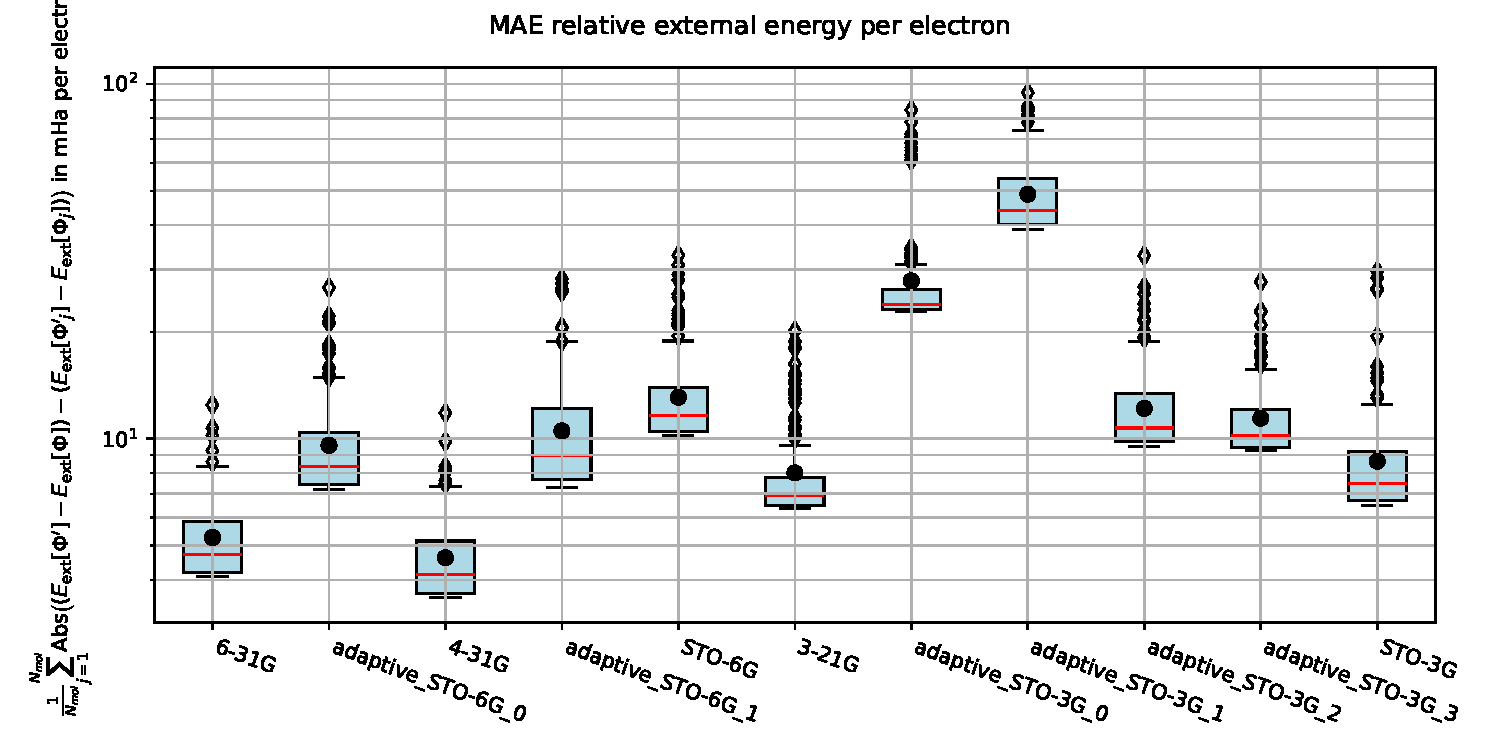
\includegraphics[width=0.9\textwidth]{chapters/results/results_images/adaptive_basis_functions/relative_coulomb_energy_adaptive_basis_sets}
    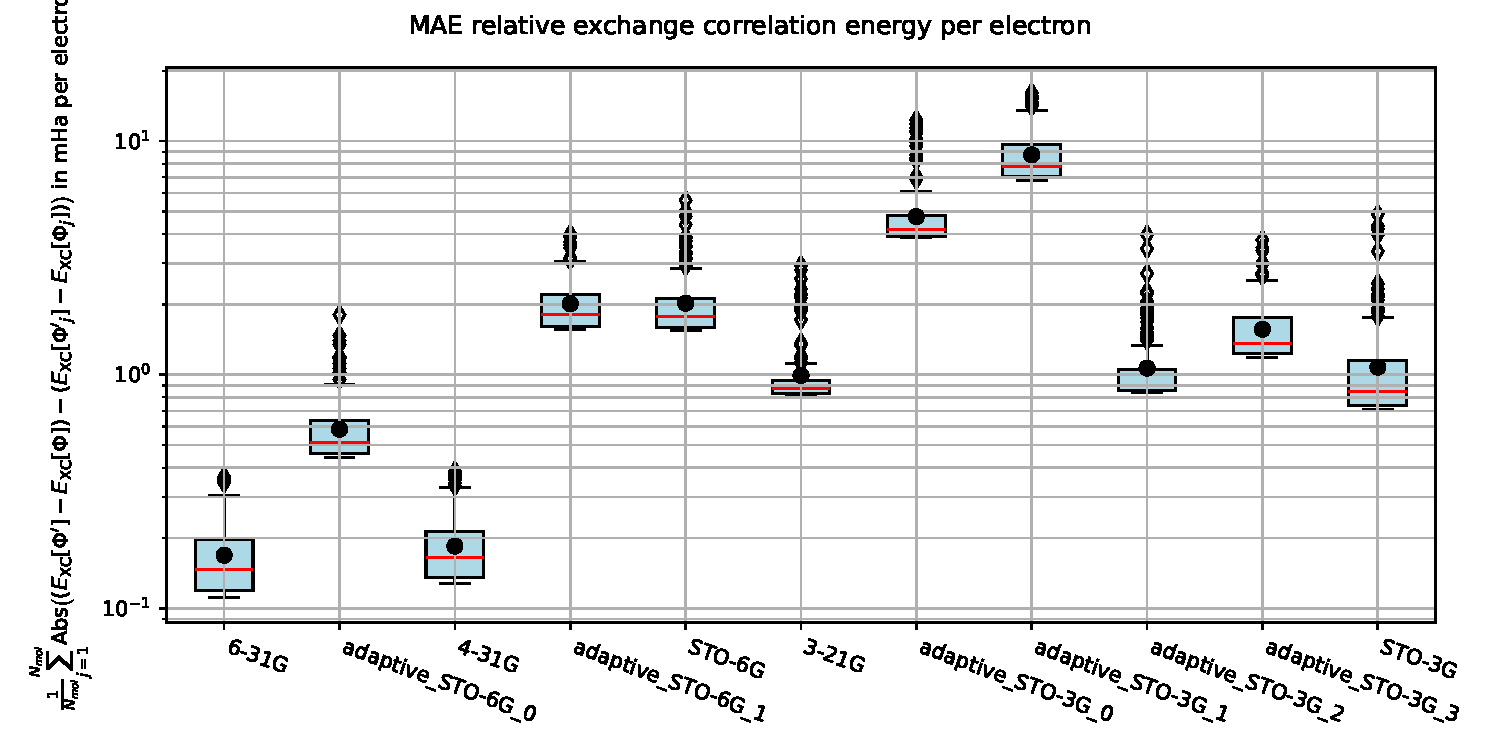
\includegraphics[width=0.9\textwidth]{chapters/results/results_images/adaptive_basis_functions/relative_exchange_correlation_energy_adaptive_basis_sets}
    \caption{Boxplots(\ref{boxplots}) of the AE for the relative energies errors(\eqref{relative_energy_errors}) produced by kohn sham on the different classical and adaptive basis functions on 210 Molecules evenly distributed over QM9, compared to calculations on the basis set "6-31G(2df,p)".}
    \label{fig:AE_relative_energies_adaptive_basis_sets}
\end{figure}
Finally we are going to compare the densities produced by the different basis sets directly. In figure \ref{fig:residual_density_adaptive_basis_sets} we show the L2 and L1 norm of the difference of the ground state density produced by the different basis sets to the density produced by 6-31G(2df,p).
As we try to predict basis functions which we can use to better reproduce the ground state orbitals of 6-31G(2df,p) one would assume that this also leads to better densities, but the opposite is true.
While the bigger basis sets produce better densities than the smaller one, do the adaptive basis functions produce consistently worse densities than their classical counterparts.
An explanation for this could be that the adaptive basis sets are optimized for fitting of the orbitals of 6-31G(2df,p), but when they are used in kohn sham calculations they deviate from these orbitals in order to minimize the total energy.\\
We can also take a look at the density directly in figure \ref{fig:adaptive_basis_set_slices} were we plotted the ground state densities of ethanol that were calculated using the different basis sets and subtracted the density produced by 6-31G(2df,p).
There we find that  the adaptive basis  for the most par show a higher and further distributed density error than the classical basis sets.\\
To compare to the recent works of Müller et. al.\cite{muller_atom--molecule_2023} and Schütt et. al.\cite{schutt_machine_2018} is not possible as they tested their adaptive basis sets on the use case of DFT calculations, which is not feasible for us as it would include calculating gradients we respect to the atom positions, which we cannot effort with the speed of our  current differentiable integrals.
\begin{figure}
    \centering
    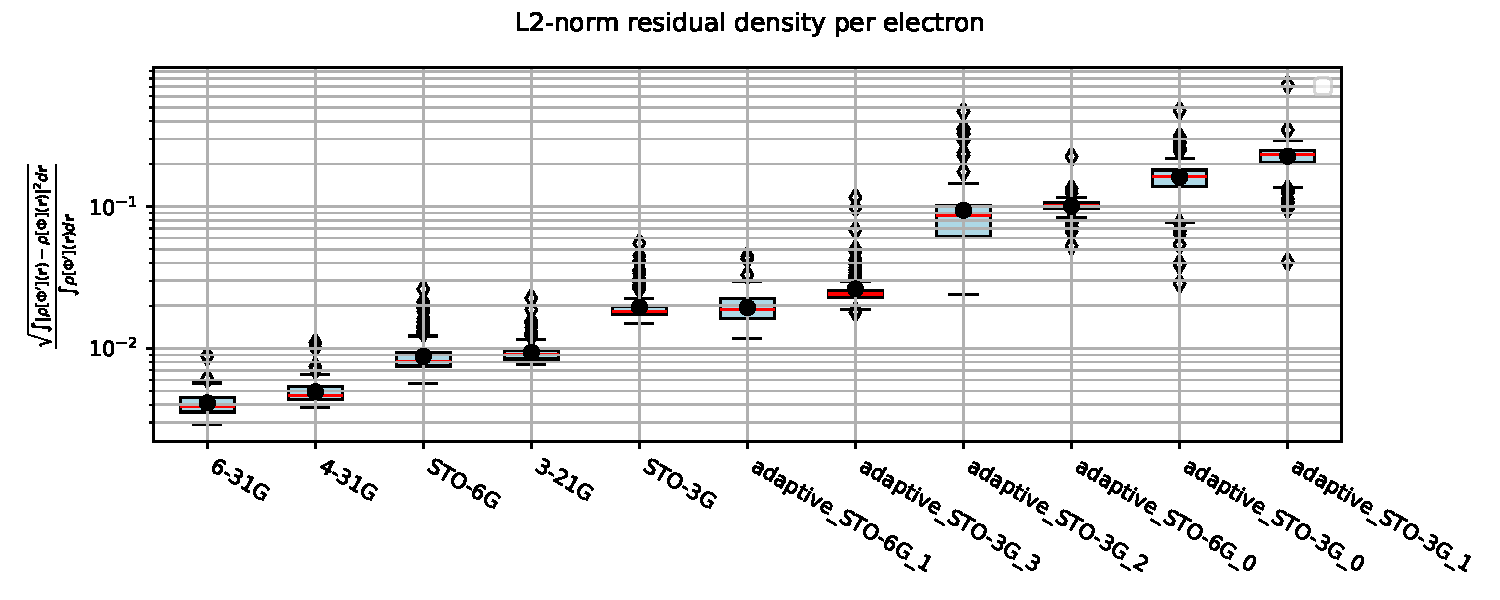
\includegraphics[width=0.9\textwidth]{chapters/results/results_images/adaptive_basis_functions/L2-norm_residual_density_per_electron_adaptive_basis_sets}
    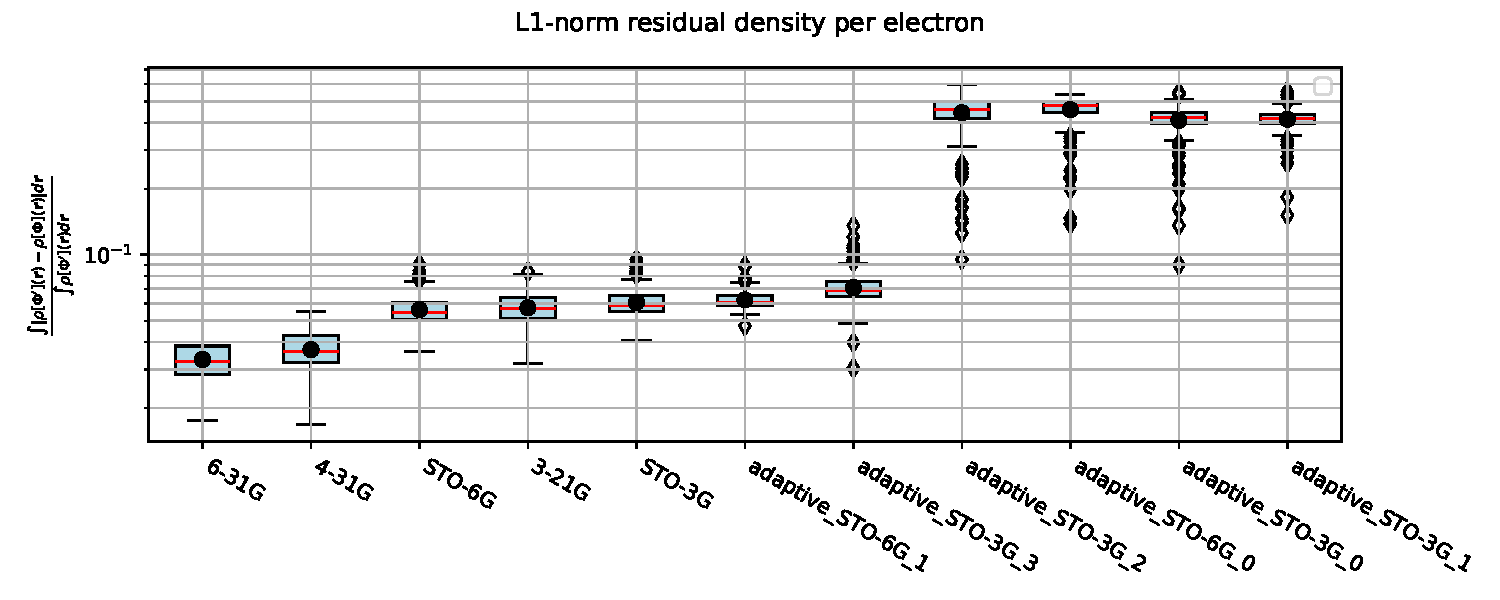
\includegraphics[width=0.9\textwidth]{chapters/results/results_images/adaptive_basis_functions/L1-norm_residual_density_per_electron_adaptive_basis_sets}
    \caption{Boxplots(\ref{boxplots}) of the difference in densities produced by kohn sham on the different classical and adaptive basis functions on 210 Molecules evenly distributed over QM9, compared to calculations on the basis set "6-31G(2df,p)".}
    \label{fig:residual_density_adaptive_basis_sets}
\end{figure}
\begin{figure}
    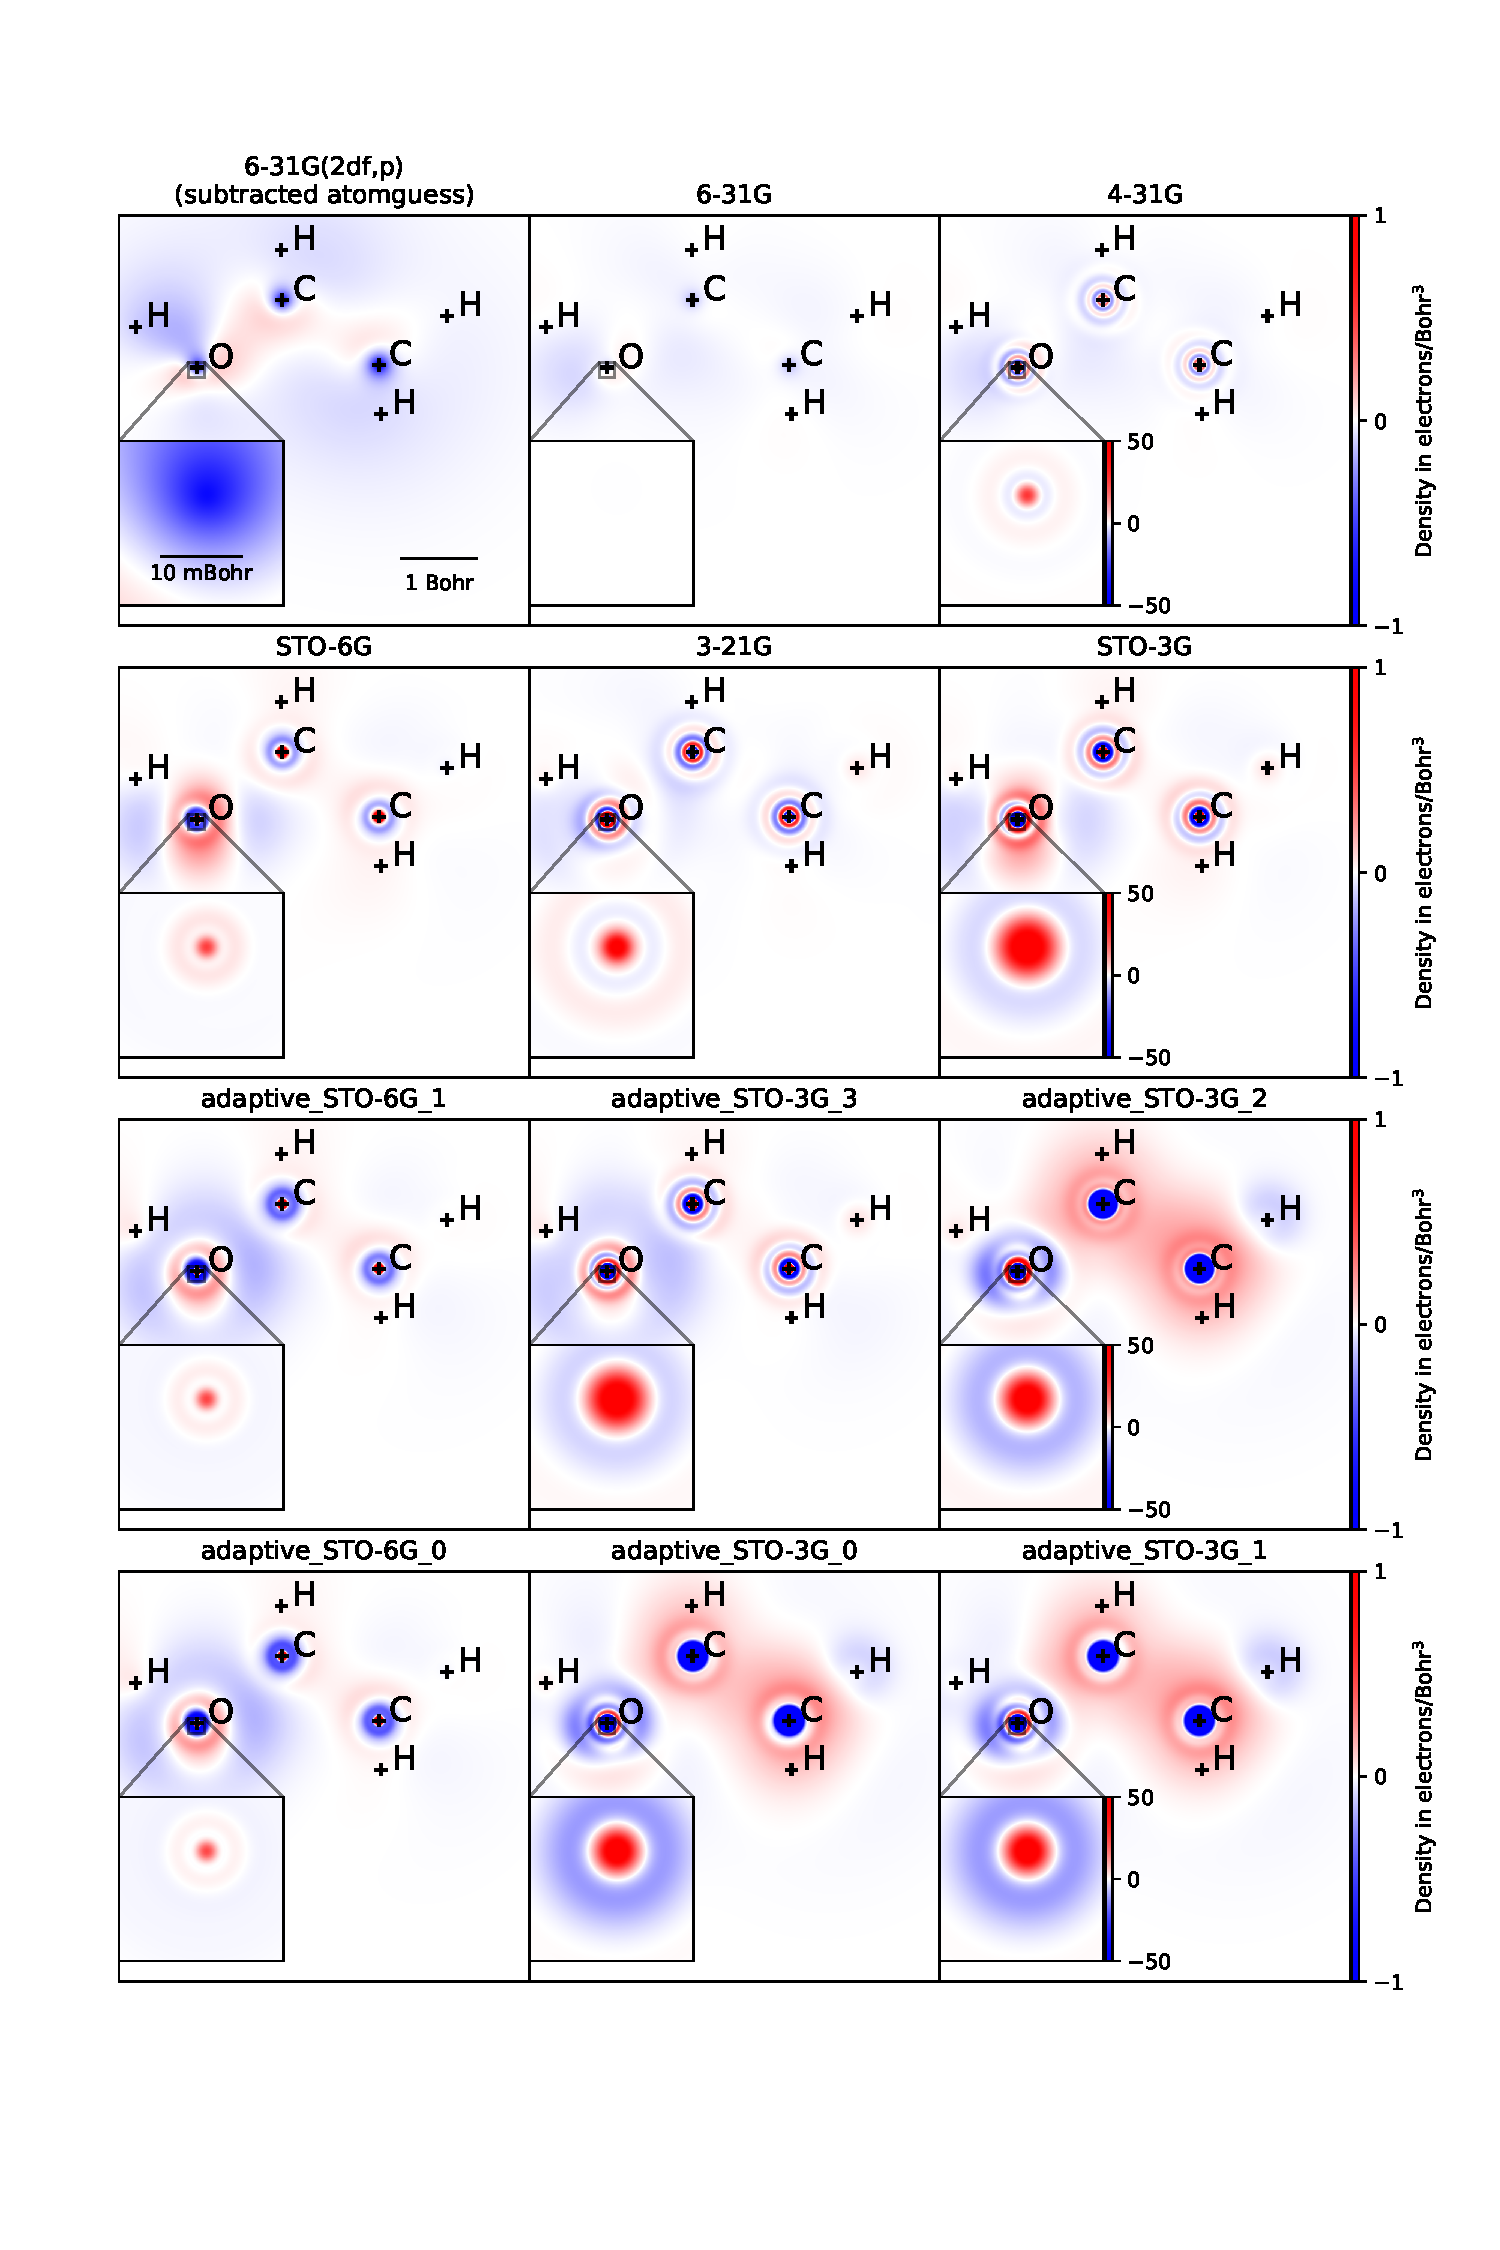
\includegraphics[trim={2cm 4.5cm 1.0cm 3.cm},clip,width=1.\textwidth]{chapters/results/results_images/adaptive_basis_functions/adaptive_basis_set_slices}
    \caption{The upper Slices of the error in the densities produced by the different basis sets on ethanol. The error is calculated as the difference of the density produced by the different basis sets to the density produced by 6-31G(2df,p).} \label{fig:adaptive_basis_set_slices}
\end{figure}
\newpage
\sections{Conclusion}
We have shown that it is possible to predict the exponents and coefficients of a minimal basis set using a small graph neural network to improve the total energy of Kohn-Sham calculations.
unfortunately we were unable to train models which would also reliably improve the external and exchange correlation energies or generate better densities.
More detailed fine tuning would be probably necessary to satisfy these additional metrics.
But nether the less we could demonstrate the potential and wide range of possible use cases for our differentiable basis functions and integrals.














